\subsection{Spielwelt}
Die grundlegende Idee der Spielwelt ist, dass diese in zwei Instanzen geteilt wird. Die erste Instanz stellt die Oberwelt dar, wo Pflanzen und Bäume wachsen, wobei die zweite Instanz den Innenraum des Bienenstocks darstellt. In dem Bienenstock können Strukturen gebaut werden, welche in der Außenwelt nicht verfügbar sind. In der Außenwelt hingegen finden sich die Ressourcen, welche für das Fortleben essenziell sind. Für die gesamte Welt, in welcher das Spiel gespielt wird, stehen mehrere Optionen der Erstellung zur Verfügung.

\paragraph{Gridless}
Die erste Möglichkeit einer Spielwelt ist eine Karte ohne dargestelltes oder vorhandenes Grid. Solch ein System verwendet beispielsweise \textit{Age of Mythology}, wobei die Karte nicht in ein Grid, sondern viele tausende  Koordinaten eingeteilt ist. Diese Form der Positionierung ist daher gängig für \textit{Realtime Strategy} Spiele.

\paragraph{Square Grid}
Eine weitere Möglichkeit zur Positionierung von Gebäuden oder Einheiten innerhalb einer Spielwelt ist ein \textit{Square Grid} (vgl. \autoref{image:squaregrid}), also die Einteilung der Karte in eine gewisse Anzahl von Quadraten, welche als eigene Felder agieren und worauf Gebäude oder Einheiten zugreifen können. Dieses System wird unter anderem in \textit{Starcraft II} oder \textit{Age of Empires} verwendet, wodurch auch diese Form der Positionierung gängig für \textit{Realtime Strategy} ist. Allerdings findet man diese Eigenschaft auch in \textit{Turn Based Strategy}, darunter die älteren Teile der \textit{Civilization}-Reihe. Dieses System wurde im Laufe der Jahre jedoch von einem Square Grid auf ein Hex Grid umgestellt.

\begin{figure}
    \begin{center}
        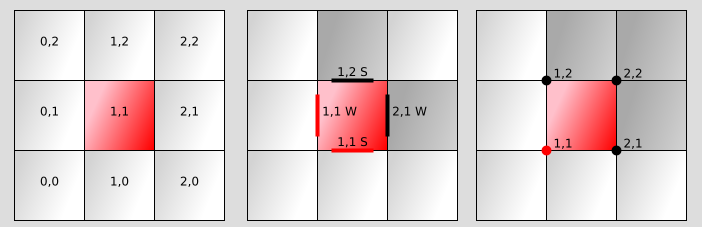
\includegraphics[width=300px]{0.bilder/squaregrid.png}
    \end{center}
    \caption{Aufbau eines Square Grids (\cite{world:grids})} \label{image:squaregrid}
\end{figure}

\paragraph{Hex Grid}
Die letzte Möglichkeit ist ein \textit{Hex Grid}, welches vor allem Anklang findet im Genre der \textit{Turn Based Strategy} Games, darunter \textit{Endless Legend}, \textit{Civilization VI} und \textit{Humankind}. Der klare Vorteil von einem Grid bestehend aus Hexagonen ist die \textit{Distanzberechnung} und die Anzahl \textit{direkter Nachbarn}. Im Vergleich zu einem Quadrat besitzt ein Hexagon in einem Grid 6 statt 4 direkter Nachbarn, wobei direkt bedeutet, dass die Kanten aneinander angrenzen. Um einen diagonalen Weg in einem Square Grid einzuschlagen, muss ein weiterer Weg aufgewendet werden, da nach dem \textit{Satz des Pythagoras} gilt:
\begin{equation}
    a^2 + b^2 = c^2
\end{equation}
Der diagonale Weg innerhalb eines Quadrates mit Länge 1 und Breite 1 wäre folglich 
\begin{equation}
    \sqrt{1^2 + 1^2} = \sqrt{2}
\end{equation}
Wobei offensichtlich gilt, dass
\begin{equation}
    \sqrt{2} > 1
\end{equation}
Möchte man also Bewegungen von Einheiten in 6 statt 4 Richtungen ermöglichen, empfiehlt sich ein Hex Grid statt einem Square Grid. Die Distanz zwischen allen gegenüberliegenden Kanten eines Hexagons ist stets gleichlang (vgl. \autoref{image:hexgrid}). Unter der Berücksichtigung, dass die Thematik der Bienen auch mit \textit{Bienenwaben} und deren hexagonalen Form assoziiert wird, wird der Prototyp ein Hex Grid verwenden. 
\begin{figure}
    \begin{center}
        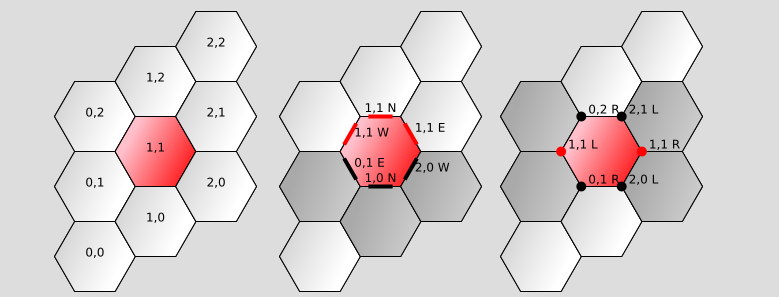
\includegraphics[width=300px]{0.bilder/hexgrid.png}
    \end{center}
    \caption{Aufbau eines Hex Grids (\cite{world:grids})} \label{image:hexgrid}
\end{figure}

\subsubsection{Generierung}
Das Terrain beziehungsweise Grid wird über einen vielschichtigen Algorithmus generiert, welcher die gesamte Fläche in Columns und die Columns wiederum in Chunks unterteilt. Der Algorithmus wurde mittels eines im Internet gefundenen Tutorials \cite*[]{world:tutorial} erarbeitet und anschließend angepasst. Mittels der Methode \textit{GenerateMap} (vgl. \autoref{code:worldgeneration}) kann von außerhalb dann der Algorithmus verwendet werden. Es gibt etliche Variationen zur Anpassung, darunter ein Seed, welcher die Generierung beeinflusst, Meeresspiegel, Erosion, Feuchtigkeit und Temperatur, es ist damit viel Diversität zwischen verschiedener Karten gegeben. In dieser Arbeit wird nicht weiter auf dieses Tutorial eingegangen, ist jedoch für weitere Informationen verlinkt. Der Bienenstock ist in dem Prototypen lediglich eine kleinere Version der generierten Außenwelt und noch nicht visuell als Bienenstock erkennbar. Dies wird in zukünftigen Iterationen angepasst und gelb und orange eingefärbt. Außerdem soll ein Ausgang für die Bienen in dem Bienenstock generiert werden, durch welchen die Einheiten sich von Bienenstock nach Außenwelt und umgekehrt bewegen können. 

\definecolor{LightGray}{gray}{0.9}
\begin{listing}[H]
\caption{World Generation}
\label{code:worldgeneration}
\begin{minted}[
bgcolor=LightGray,
framesep=2mm,
baselinestretch=1.2,
fontsize=\footnotesize,
linenos,
]{csharp}
public void GenerateMap (int x, int z, bool wrapping) {
    Random.State originalRandomState = Random.state;
    if (!useFixedSeed) {
        seed = Random.Range(0, int.MaxValue);
        seed ^= (int)System.DateTime.Now.Ticks;
        seed ^= (int)Time.unscaledTime;
        seed &= int.MaxValue;
    }
    Random.InitState(seed);

    cellCount = x * z;
    overworldGrid.CreateMap(x, z, wrapping);
    if (searchFrontier == null) {
        searchFrontier = new HexCellPriorityQueue();
    }
    for (int i = 0; i < cellCount; i++) {
        overworldGrid.GetCell(i).WaterLevel = waterLevel;
    }
    CreateRegions();
    CreateLand();
    ErodeLand();
    CreateClimate();
    CreateRivers();
    SetTerrainType();
    for (int i = 0; i < cellCount; i++) {
        overworldGrid.GetCell(i).SearchPhase = 0;
        overworldGrid.GetCell(i).MapType = HexMapType.Overworld;
    }

    Random.state = originalRandomState;
}
\end{minted}
\end{listing}